%-----------------------------------------------------------------------------------------------
\chapter{Marker Recognition}\label{sect:marker_recognition}
%-----------------------------------------------------------------------------------------------

The preprocessing steps used for preparing the images for the line fitters (segmentation, thresholding, filtering etc.) will also be discussed.

The input is the raw image taken\footnote{In the development phase rendered pictures were used for better repeatability} by the observer.
The first problem is finding the RQIM on the picture.
When the marker area is located, it is necessary to discard the only partially visible and/or unrecognisable quads.
At this point there is an image or set of images containing potentially good quads.

%-----------------------------------------------------------------------------------------------
\section{Preprocessing}
%-----------------------------------------------------------------------------------------------

The preprocessing is done in two stages.
The first is the segmentation, when quad-like blobs are found.
The second step is the preparation of the aforementioned blobs for the line fitting algorithms' needs.

%-----------------------------------------------------------------------------------------------
\section{Segmentation}
%-----------------------------------------------------------------------------------------------

The segmentation process is carried out on images roughly like the one shown in figure \figref{partialMarkerShot}.
First the photos are converted to binary format by applying a threshold.
The image is inverted in the process, because it makes more sense for the objects to be marked with non-zero elements than vice-versa.
The threshold's value is determined using Otsu's method, which maximises the inter-class variance of the clusters\footnote{Foreground and background}.
The implementation is provided by the OpenCV framework.

Afterwards, the binary image is conditioned with a \emph{close} morphology operator.
The closing removes the gaps from the large connected areas (possible quads) and removes the \emph{salt and pepper}-like noise.
In the current implementation the kernel size of the morphology operator is constant, however it could be beneficial to calculate it from the global or local image parameters\footnote{e.g. image size, area of the connected region, etc.}.

The segmentation is based on finding continuous contours on the binary image.
The OpenCV framework provides great functionality for this.
The implementation is based on calculating the 8-neighbour chain code for the binary blobs on the image.
The functions returns a list of list of points for the borders os each distinct contour.

The next step is the filtering of the found blobs.
First the surely partial quads are discarded.
This is done by calculating the bounding box of the contours, and if one of it's sides are touching the image border, the blob is marked as partial.
With this approach it is possible that some fully visible quads that only touch the image border with one of their corner are lost.
This problem can be easily fixed by checking the neighbourhood of the contact point, but this is not yet implemented.

\begin{figure}[ht]
	\begin{subfigure}{0.3\textwidth}
		\centering
		
\includegraphics{figures/quad3.png}
	\end{subfigure}
	\begin{subfigure}{0.3\textwidth}
		\centering
		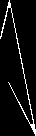
\includegraphics{figures/quad4.png}
	\end{subfigure}
	\begin{subfigure}{0.3\textwidth}
		\centering
		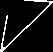
\includegraphics{figures/quad5.png}
	\end{subfigure}
	\caption{Quad candidates after segmentation}
	\label{fig:segmentationOutput}
\end{figure}

The next blob-filtering step is to filter out the false-positive contours.
These false hits can be caused by the light conditions or the scene around the marker.
For this purpose a simple metric is used to measure how likely a blob is to be a quad. 
This metric is the ratio of a blob's area and circumference. 
By experimentation this ratio for quads is found to be in the range of 10 and 50.
The contours with ratios outside these limits are discarded.

The segmentation processes output is available as a singe image with colour-coded\footnote{Gray level, to be exact} blobs or as a list of separate images each containing a quad candidate.
Figure \figref{segmentationOutput} shows an example for the output of the segmentation process.